\chapter{Cliente}
\section{Introducción}
Se ha diseñado el cliente con una interfaz gráfica para simplificar el manejo de la aplicación distribuida al cliente. Cuando el cliente desea realizar una petición al servidor, éste invoca al proxy y el proxy realiza la petición al servidor. Cuando el servidor acaba, el resultado le llega al cliente mediante el proxy.

\section{Ejecución de la aplicación}
Una vez que se ejecuta la aplicación, lo primero que pide es la IP del servidor tal y como se ve en la figura \ref{fig:elegir_ip}
\begin{figure}[htb]
	\centering
	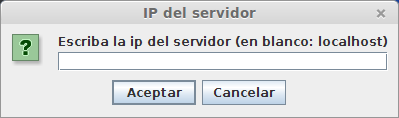
\includegraphics[scale=1]{imagenes/elegir_ip.png}
	\caption{Elegir IP}
	\label{fig:elegir_ip}
\end{figure}
Una vez introducida la IP se ejecuta la ventana principal de la aplicación.

\subsection{Ventana principal}
La ventana principal (ver figura \ref{fig:main_gui}) consta de una barra de menú y de cuatro botones:
\begin{itemize}
	\item Subir fichero: sube un fichero al servidor.
	\item Descargar fichero: descarga un fichero al cliente.
	\item Sincronizar reloj: Sincroniza el reloj del cliente con el del servidor.
	\item Actualizar directorios: Actualiza los directorios (remoto y local).
\end{itemize}

\begin{figure}[htb]
	\centering
	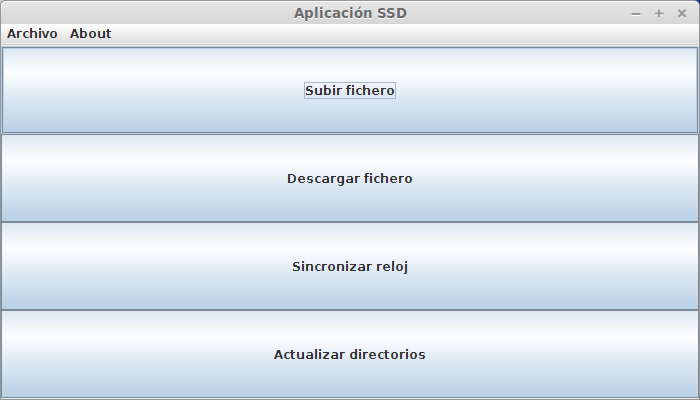
\includegraphics[scale=0.7]{imagenes/main_gui.png}
	\caption{Ventana principal}
	\label{fig:main_gui}
\end{figure}

\hspace*{-5mm} El contenido de la barra de menú es el siguiente:
\begin{itemize}
	\item Archivo
	\begin{itemize}
		\item Ajuestes
		\begin{itemize}
			\item Cambiar carpeta local: cambia la carpeta local
			\item Cambiar carpeta remota: cambia la carpeta remota (ver figura \ref{fig:remote_folder_gui})
			\item Cambiar Tmin: cambia el tiempo mínimo de transmisión de un paquete del cliente al servidor
		\end{itemize}
		\item Salir: cierra la aplicación
	\end{itemize}
	\item About
	\begin{itemize}
		\item Carpeta local: muestra la ruta de la carpeta local.
		\item Tmin: muestra el valor del tiempo mínimo de transmisión de un paquete del cliente al servidor
		\item Información: muestra la información acerca de la aplicación
	\end{itemize}
\end{itemize}

\begin{figure}[htb]
	\centering
	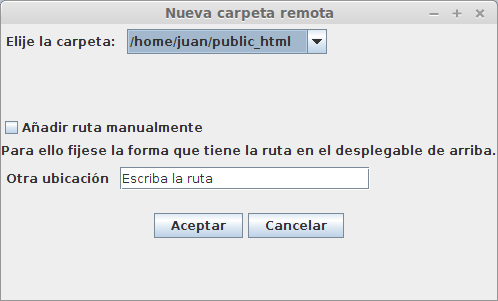
\includegraphics[scale=0.7]{imagenes/remote_folder_gui.png}
	\caption{Elegir directorio remoto}
	\label{fig:remote_folder_gui}
\end{figure}

\subsection{Elegir directorio remoto}
Como se puede observar en la figura \ref{fig:remote_folder_gui}, la ventana consta de dos partes.\\ La primera parte contiene un desplegable con todas las posibles carpetas (existentes) del servidor que pueden ser la nueva carpeta remota.
\\Si por algún motivo se quisiese elegir otra carpeta en la segunda parte se ha creado un campo de texto para introducir la ruta. \\Cuando se le da al botón de aceptar, por defecto escoge la ruta de la primera parte. Si se quiere poner una ruta manualmente es necesario activar la casilla que hay justo encima para que la ruta que se pase al servidor sea la ruta manual.
